\documentclass{article}
\usepackage{graphicx} % Required for inserting images
\usepackage{subcaption}
\usepackage{amsmath, amsfonts}
\usepackage[a4paper, total={6.5in, 10in}]{geometry}
\usepackage[round]{natbib}
\bibliographystyle{unsrtnat}
\usepackage{hyperref}

\title{PREDICTING FOREST FIRES \\ 
A guide to using machine learning models to predict forest fires and understand their causes}
\author{}
\date{}

\begin{document}

\maketitle

\section{Introduction}

This report will examine how best to predict forest fires, based on the Forest Fires data set from the UCI machine learning repository. It contains 517 instances of the area of forest fires, along with a selection of 12 explanatory features.

Naturally, as with any natural disaster, being able to predict areas where forest fires are likely to break out and identifying which variables contribute to an increased risk of forest fire would allow resources to be spent at the right times and locations, potentially saving lives and nature. In the following sections, this report explores the dataset and its variables, introduces the machine learning models used to predict forest fires, and discusses the most important findings and takeaways.

\section{Data \& exploration}

The data was collected at the Montesinho Natural Park, located at the northern border of Portugal. The target variable \texttt{area} ranges from 0.0 to 1090.84 and measures the area of the fire in hectares (ha). The variables \texttt{X} and \texttt{Y} range from 1 to 9 and 2 to 9, respectively, and locate the fire on the Montesinho Natural Park map, as depicted in figure \ref{fig:map_fires} below. The fires are located with some added jitter in the middle of the coordinate squares, and the size indicates the area burned.

\begin{figure}[!htbp]
    \centering
    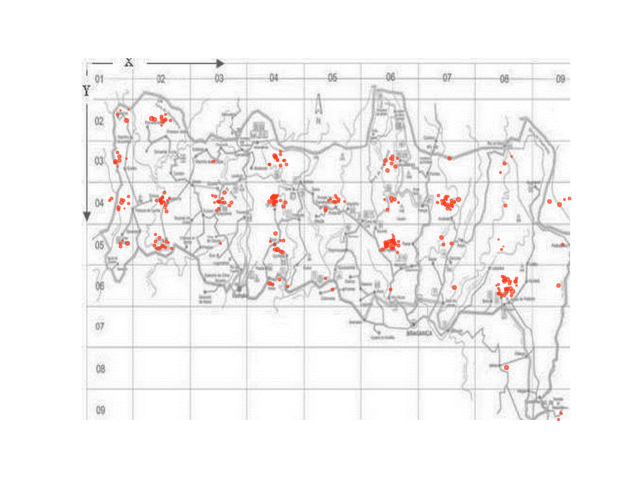
\includegraphics[width=0.85\textwidth]{map_fires.png}
    \caption{Map of fires in Montesinho Natural Park}
    \label{fig:map_fires}
\end{figure}

The variables \texttt{month} and \texttt{day} are categorical and denote the month (`jan' to `dec') and day (`mon' to `sun') of the incident.
The variables \texttt{FFMC}, \texttt{DMC}, \texttt{DC} and \texttt{ISI} all come from the Forest Fire Weather Index (FWI), which comprises of several different metrics and measures the risk of wildfire incidents. \texttt{FFMC} (Fine Fuel Moisture Code) measures the humidity/moisture of litter and other small components that could fuel a fire, \texttt{DMC} (Duff Moisture Code) relates to the moisture of larger components, \texttt{DC} (Drought Code) measures the humidity of deeper layers of the environment, and \texttt{ISI} (Initial Spread Index) is a measure of the wind which would help a fire spread.
The variables \texttt{temp} and \texttt{RH} measure temperature (in Celcius) and relative humidity (in \%), respectively, while \texttt{wind} measures wind speed in km/h and \texttt{rain} denotes rain in mm/m$^2$.

\paragraph{Processing} To feed the data to machine learning models, some processing needs to be done. The variables \texttt{month} is categorical and in string-form and will be recoded as integers, ranging from 1 to 12. Similarly, \texttt{day} will be recoded to an integer in 1 to 7. Moreover, the target variable \texttt{area} is heavily skewed towards 0 and will be transformed through $\texttt{area} = \ln(\texttt{area} + 1)$, as done in the original paper by \cite{origpaper}. This transformation ensures that the data appears less skewed and has less extreme outcomes. To inspect the final predicted outcomes, the inverse of $\ln(x+1)$ is taken, which is $e^{x} - 1$.

Figure \ref{fig:hist_area} shows the histograms of the outcome variable before and after transformation. While the area had values above 1000, the (natural) log-transformation has maximum values only around 7. While the majority of observations are still at or around 0, there are more observations around values 1-4, which should help model predictions.

\begin{figure}[!ht]
\centering 
\begin{subfigure}{0.48\textwidth} 
    \centering 
    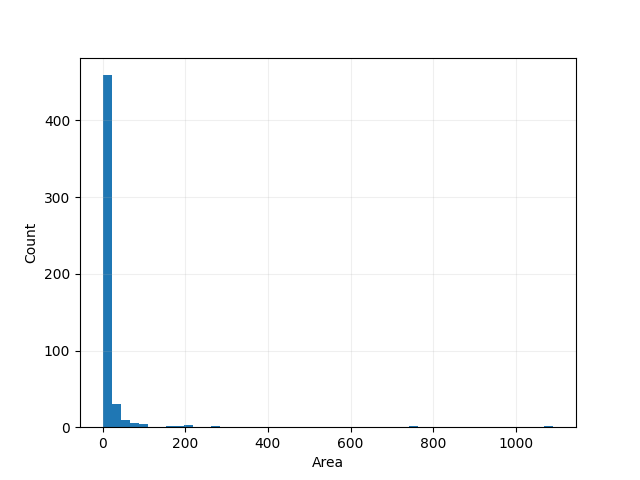
\includegraphics[width=1.05\linewidth]{hist_orig.png} 
    \caption{Original area} 
    \label{fig:hist_orig} 
\end{subfigure} 
\begin{subfigure}{0.48\textwidth} 
    \centering
    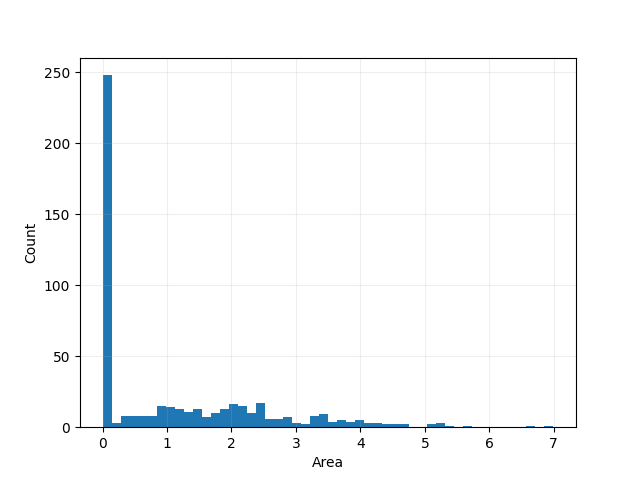
\includegraphics[width=1.05\linewidth]{hist_transformed.png} 
    \caption{log-transformed area} 
    \label{fig:hist_transformed} 
\end{subfigure}
\caption{Histograms of the outcome variable \texttt{area} before and after transformation}
\label{fig:hist_area}
\end{figure}

To investigate which variables seem to be related to the area, we can turn to pairwise scatterplots of the outcome variable against all other variables.

\begin{figure}[!htbp]
    \centering
    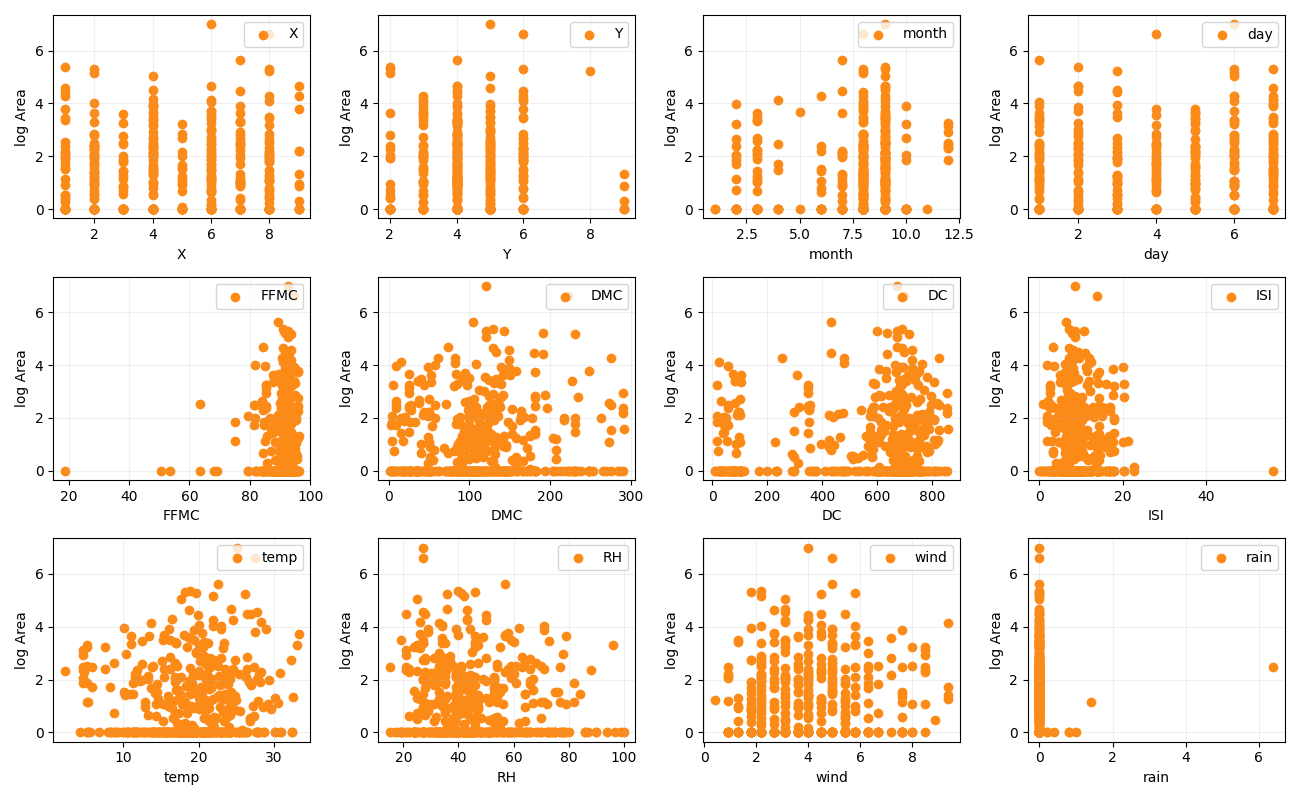
\includegraphics[width=0.95\textwidth]{all_scatters.png}
    \caption{Scatter plots of outcome against all feature variables}
    \label{fig:all_scatters}
\end{figure}

Looking at the scatterplots in figure \ref{fig:all_scatters}, the majority of features do not show a clear relation with the outcome although it seems that the outcome goes up with increasing months or temperatures. To investigate how variables are correlated with each other and the outcome, a correlation heatmap can be used.

\begin{figure}[!htbp]
    \centering
    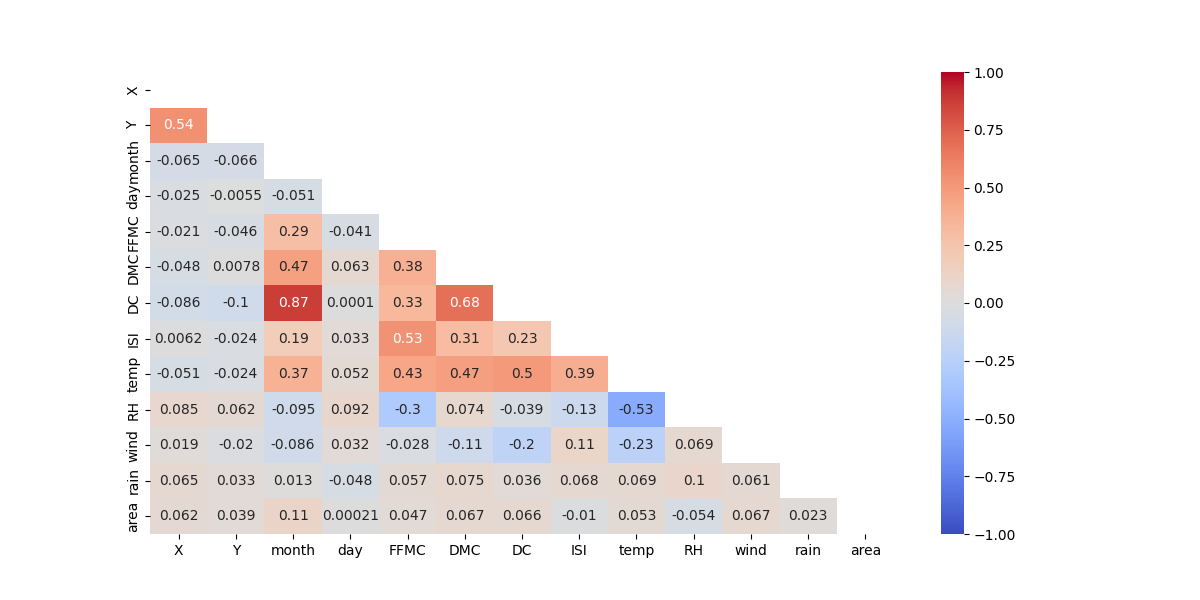
\includegraphics[width=\textwidth]{corr_heatmap.png}
    \caption{Correlation heatmap}
    \label{fig:corr_heatmap}
\end{figure}

Interestingly, the majority of variables do not show any correlation amongst each other and with the area (before transformation). However, the month and temperature are correlated positively with each other and all of the four indicators from the Forest Fire Weather Index (\texttt{FFMC}, \texttt{DMC}, \texttt{DC} and \texttt{ISI}). All of those indicators are also positively correlated amongst themselves, although the highest correlation (0.87) was between \texttt{DC} and \texttt{month}. Moreover, correlations with the outcome \texttt{area} are very small in magnitude for all variables.

\section{Models \& methodology}

To try and predict the area of forest fires, I will use a simple linear regression, random forest, XGBoost, a Gaussian process a generalized linear model for gamma distributed outcomes. Those models have all been widely and successfully used in the literature.

\paragraph{Linear Regression} Linear regression, based on ordinary least squares (OLS) is a relatively simple model to model the relationship between target $y$ and predictors $X$, where $X$ denotes the design matrix of variables and intercept, and all observations. The target variable is assumed to have a normal distribution with variance $\sigma^2$ and mean $X\beta$ and can thus be expressed as

\begin{equation}
    \label{eq:ols}
    y = X\beta + \epsilon,
\end{equation}

where each $\epsilon_i$ has variance $\sigma^2$ and thus $y_i \sim \mathcal N(x_i\beta, \sigma^2)$. The estimate of coefficient vector $\beta$ is $\hat \beta = (X'X)^{-1}X'y$. The advantage of the OLS estimator $\hat \beta$ is that it can easily be interpreted as partial effects of the variables and leads to interpretable results.

\paragraph{Gaussian Process} 
Gaussian Processes (GPs) are a powerful, non-parametric Bayesian technique that can be used for regression tasks. At its core, a Gaussian Process is an infinite collection of random variables, any finite number of which have a joint multivariate Gaussian distribution. In the context of machine learning, GPs are used to model the function that maps inputs to outputs. The key idea is that instead of assuming the function is known up to a finite-dimensional parameter vector (as in parametric methods), GPs assume the function is drawn from a prior distribution that is Gaussian. This means that the function itself is left unspecified, allowing any kind of function, making them particularly useful in scenarios where the underlying process is complex and the data is limited. By placing a Gaussian prior over the function space, GPs can predict not just the mean of the output variable, but also its variance, giving a measure of the uncertainty in the prediction. The GP assumes a prior zero mean, so the outcome variable should be standardized, as performance deteriorates greatly otherwise. The package \texttt{sklearn.gaussian\_process.GaussianProcessRegressor} natively implements the standardization through a keyword. The most important part of a GP is the covariance function, which essentially determines the distance between observations and thus how new predictions are formed based on previously observed values. I chose the default option of a constant kernel, multiplied with an RBF (also known as squared exponential) kernel, defined as $k_{RBF}(x_i, x_j) = \sigma^2_f\exp\left(-\frac{(x_i - x_j)^\top(x_i - x_j)}{l^2}\right),$ with $l$ the length scale and $\sigma^2_f$ the amplitude. The optimal parameters are automatically found by optimizing the log marginal likelihood \citep{schulz2018tutorial}.

\subsection*{Tree-based models}
\paragraph{Random Forest}
Random Forests (RF) are an ensemble learning method that operates by constructing multiple decision trees during training and outputting the mean prediction of the individual trees. By training a multitude of decision trees on various sub-samples of the dataset and using averaging to improve the predictive accuracy and control over-fitting, RFs offer robust predictions \citep{rfs}. This model can be implemented easily with the class \texttt{sklearn.ensemble.RandomForestRegressor}.

\paragraph{XGBoost} XGBoost, short for eXtreme Gradient Boosted trees, is a very successful machine learning model. It operates by combining the predictions from several trees and is thus an ensemble model. Contrary to e.g. a Random Forest, trees are trained in a sequential manner, where each additional tree in the ensemble is trained to predict the residual error of the ensemble of previous trees. Moreover, the predictions from each tree are scaled by a factor $\nu$ (typically below 0.1) to improve generalization and reduce overfitting \citep{xgb}. This model is implemented in the class \texttt{xgboost.XGBRegressor}.

\paragraph{Hyperparameter tuning}
Both RF and XGBoost have hyperparameters that have to be tuned to obtain the best results. Because a wide range of values are possible for each hyperparameter, a grid search would have to be extremely sparse or is entirely unfeasible computationally, so I used Bayesian Optimization (BO) to find the best set of hyperparameters, which leverages Bayesian inference to construct a GP model of the objective function (MSE on a validation set, given the hyperparameter values), allowing for efficient exploration and exploitation of the search space. This GP model predicts the expected outcome and uncertainty of the objective function at any given point in the search space. By iteratively selecting the next point to evaluate based on maximizing the expected improvement or acquiring the most information, BO finds the optimal solution with fewer evaluations compared to e.g. grid search \citep{BO}. For RF, the parameters are the number of trees  \texttt{n\_estimators} (optimal value 126), the maximum depth for each tree \texttt{max\_depth} (2), the maximum subset of features to use at each split \texttt{max\_features} (0.7721) and the minimum number of samples in a leaf node required to allow a split \texttt{min\_samples\_split} (2). For XGBoost, the hyperparameters to tune are also \texttt{n\_estimators} (279) and \texttt{max\_depth} (4), the subset of observations to use at each iteration \texttt{subsample} (0.6591) and the learning rate $\nu$ (\texttt{learning\_rate}, optimal value 0.0047). 


\paragraph{Generalized linear model}
So far, all models above either do not or only implicitly assume the data distribution and might hence not be optimally suited.
The first step is to determine the likely data distribution. Looking at figure \ref{fig:hist_area}, the outcome is heavily right-skewed and continuous, so possible target distributions are Gamma, Beta, Weibull, Exponential or Log-Normal. One way to test whether data comes from a given distribution is the Kolmogorov-Smirnov test, which compares the theoretical CDF $F_0(x)$ with the empirical CDF $\hat F_n(x)$, as described in \cite{ks}. The test statistic is given by 

\begin{equation}
    \label{eq:kstest}
    D_n = \sup_{x\in \mathbb R} |\hat F_n(x) - F_0(x) |,
\end{equation}

where $\hat F_n(x) = \frac{1}{n} \sum_{i=1}^n 1_{(-\infty, x]}(X_i)$. The corresponding p-value can then be obtained for desired confidence level, given sample size $n$. 

Applying this methodology to the outcome variable \texttt{ln(area)}, the best fit is the Gamma distribution with parameters $\alpha = 0.4$ and scale $\theta = 1$. Still, the p-value was extremely low, indicating that this best fit is likely still not the true data distribution.
Figure \ref{fig:gamma_dist} below shows a histogram of the true outcomes along with the density. While the density fits reasonably well and displays the spike for outcomes around 0, it does not accurately fit the tail of the distribution.

\begin{figure}[!htbp]
    \centering
    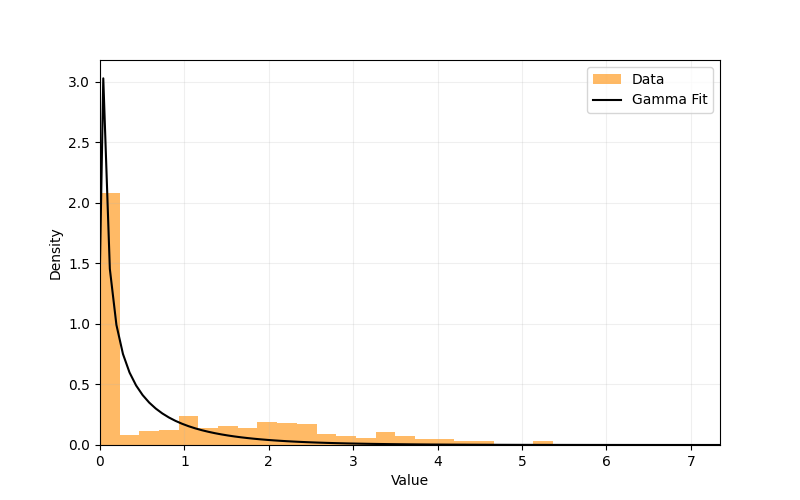
\includegraphics[width=0.9\textwidth]{data_gamma_dist.png}
    \caption{Outcome variable with density plot of best-fitting distribution}
    \label{fig:gamma_dist}
\end{figure}

Assuming a gamma distribution for the outcome, a general linear model can be employed, which takes this distribution into account \citep{glm}. The package \texttt{sklearn.linear\_model.GammaRegressor} can then be used to predict the outcome as a function of the predictors. Because the data has strictly non-negative values, the log-link is used, meaning predictions are formed as $\hat y_i = \exp (\beta_0 + \beta_1 x_{1i} + ... + \beta_k x_{ki} )$. Note that the negative-inverse link could also be used for the Gamma distribution. Additionally, the package includes a tuneable penalty term (also named $\alpha$) to avoid overfitting. As this is a single parameter, a standard grid search can be employed to find the parameter which performs best. Because the dataset is relatively small, dividing the training set into smaller training and validation sets might make the results highly dependent on the split chosen. To circumvent this, I use cross validation, which (for each value of $\alpha$) calculates the MSE for each of 5 folds and returns the average. That way, the results do not depend on a specific split. Figure \ref{fig:gridsearch_glm} shows the average MSE for 5 folds for each value of $\alpha$, along with the best value of around 2.6, indicating light penalization of model coefficients.

\begin{figure}[!htbp]
    \centering
    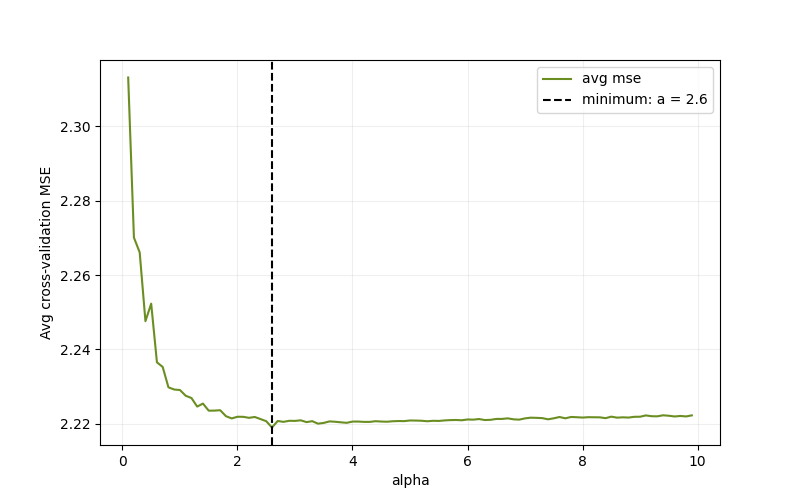
\includegraphics[width=0.9\textwidth]{gridsearch_glm.png}
    \caption{Average MSE for 5-fold cross validation for values of $\alpha$}
    \label{fig:gridsearch_glm}
\end{figure}

\subsection{Model performance}

All models above have been fit and tuned exclusively on the training set, which used 80\% of observations. All the tuning was done by either subdividing the training set into another training and validation set, or cross validation on the training set. To compare the predictive performance, the hold-out test set is used. This separation of training and test set is vital to ensure that the scores of the models reflect performance on unseen data. To later predict the area of forest fires and identify high-risk areas/cases, the best model should be used.

\begin{table}[!htbp]
\centering
\caption{MSE and MAE on the test set for all models}
\label{tab:msemae}
\begin{tabular}{lccccc}
\hline
                & \multicolumn{5}{c}{\textbf{Model}}                                                    \\ \cline{2-6} 
\textbf{Metric} & \textbf{OLS} & \textbf{Gaussian Process} & \textbf{Random Forest} & \textbf{XGBoost} & \textbf{Gamma Regressor} \\ \hline
MSE             & 1.594        & 1.556                     & 1.568                   & 1.503     & 1.584       \\
MAE             & 1.107        & 1.077                     & 1.092                   & 1.039     & 1.114      \\ \hline
\end{tabular}
\end{table}

Interestingly, the best MSE and MAE was achieved by XGBoost, followed by the Gaussian Process, although the RF is very close behind. OLS (when trained on standardized data) has a very intuitive way of analyzing the coefficients as partial effects, while XGBoost and RF also have built-in feature importance methods.

\section{Causes of forest fires}
To investigate how the different variables affect the area of a forest fire, we can first look at the coefficients of the OLS model. Note that these are coefficients for the model trained on standardized inputs, so larger coefficients directly correspond to a larger influence on the outcome. In practice, training on standardized versus unstandardized features has no impact on predictive performance, as any scaling can be absorbed in the coefficients.

\begin{table}[!htbp]
\centering
\caption{Coefficients from the OLS model trained on standardized data}
\label{tab:olscoef}
\resizebox{\textwidth}{!}{%
\begin{tabular}{lccccccccccccc}
\hline
\textbf{}      & \multicolumn{13}{c}{\textbf{Feature}}   \\ \cline{2-14} 
\textbf{} & \textbf{intercept} & \textbf{X} & \textbf{Y} & \textbf{month} & \textbf{day} & \textbf{FFMC} & \textbf{DMC} & \textbf{DC} & \textbf{ISI} & \textbf{temp} & \textbf{RH} & \textbf{wind} & \textbf{rain} \\ \hline
Coef            & 1.175***              & 0.1212 &    -0.0375 &     0.4379** &     0.0089 &    -0.0259 &     0.1749 &    -0.4049 &    -0.0233 &     0.0804 &    -0.0224 &     0.0541 &     0.0195         \\
p-value            & 0.000              & 0.1798 &     0.6592 &     0.0106 &     0.8964 &     0.3736 &     0.1587 &     0.1651 &     0.5231 &     0.1980 &     0.4527 &     0.3168 &     0.6229         \\\hline
\multicolumn{14}{l}{\footnotesize{Note: *** significant at 1\% level, ** significant at 5\% level, * significant at 10\% level}}
\end{tabular}%
}
\end{table}

Positive coefficients of the features indicate that an increase in the variable also increases the area of the forest fire. Interestingly, the coefficient of rain is positive, which one wouldn't expect. However, the coefficient is not significant and there are a lot of values in a cloud for very low values of rain, meaning that the line of best fit (so the value of the coefficient) is relatively arbitrary as the data does not show a linear trend. Apart from month, only the intercept is statistically significant, meaning that the majority of features are not very useful in predicting the area. Figure \ref{fig:coefs_ols} shows the coefficients as a bar plot. The largest coefficients are the intercept and month, although DC (which measures the humidity of deeper layers of the environment) also has a comparatively large value, with a negative coefficient.

\begin{figure}[!htbp]
    \centering
    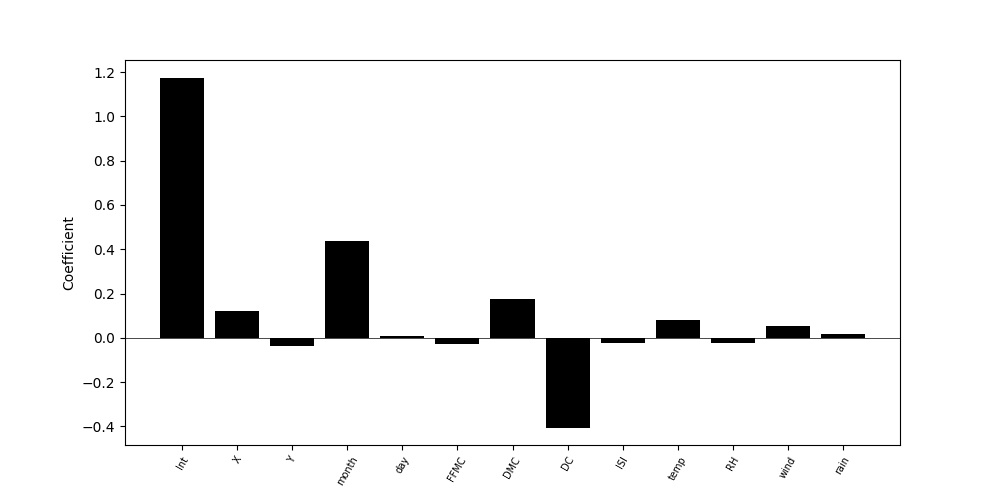
\includegraphics[width=0.85\textwidth]{coefs_ols.png}
    \caption{Coefficient estimates from OLS}
    \label{fig:coefs_ols}
\end{figure}

One problem of just analyzing the coefficients of the linear regression is the enforced linearity. Looking at the fires on the map, they seem to increase as \texttt{Y} increases first, but then decrease again for higher values because the park only stretches down into coordinate 7 for most of the area. Moreover, most fires would be expected in the summer months, with less during November or December again, but this is not possible to model with a linear regression (cross-terms or squares could be added but with relatively few observations this could harm the fit further).

Turning to the XGBoost and RF models, it's possible to investigate how often a variable was used in splits during the training process, indicating relative importance of that variable. Figure \ref{fig:fis} shows these importances.
\begin{figure}[!htbp]
    \centering
    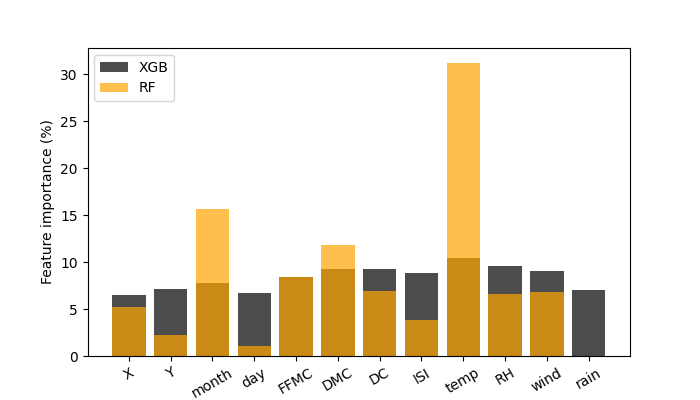
\includegraphics[width=0.85\textwidth]{FIs.png}
    \caption{Feature importances for of XGB and RF}
    \label{fig:fis}
\end{figure}
While temperature has the highest feature importance for both models, its importance is much larger for the random forest. For XGBoost, the feature importances are relatively equal, which makes more sense as the maximum depth for XGBoost is higher, so more features can be used. The variables with the lowest importances are \texttt{X}, \texttt{Y} \texttt{day} and \texttt{rain}, which intuitively makes sense as the day of the week is much less important than e.g. the month of the year and looking at Figure \ref{fig:map_fires}, the fires seem to be spread out relatively evenly across the coordinates. As mentioned above, \texttt{rain} does not show a clear relation to the outcome variable and it makes sense that it has a lower feature importance as well.

Instead of reducing each variable to a single coefficient or measure of importance, the Individual Conditional Expectation (ICE) plot shows the relation of the predicted area and a feature of interest. A Partial Dependence Plot (PDP) is the average of individual ICE lines (one per observation). This allows us to see how the predicted area of a fire changes as the variable changes from its minimum to maximum value. Roughly following the \href{https://scikit-learn.org/stable/modules/partial_dependence.html}{notation of the \texttt{sklearn} library}, denote $X_i$ as all observations of feature $i$, $x_i$ individual observations, and $X_{-i}$ all other features except $i$ (its complement) and $x_{-i}$ observations of $X_{-i}$. Then, the partial dependence of a function $f$ (here the predictive function of XGBoost) at point $x_i$ is defined as

\begin{equation}
    \label{eq:pdp}
    pd_{X_i}(x_i) = \mathbb E_{X_{-i}} [f(x_i, X_{-i})] = \int f(x_i, x_{-i})p(x_{-i}) dx_{-i}.
\end{equation}

In practice, this can be calculated as 

\begin{equation}
    pd_{X_i}(x_i) \approx \frac{1}{n} \sum_{j=1}^n f(x_i, x_{-i}^{(j)}).
\end{equation}

Note that $x_i$ here denotes a point of feature $X_i$. To obtain the whole plot, $x_i$ is varied from the minimum to maximum value, to obtain the model predictions given the changing feature value. Each orange ICE line is based on one sample (where $x_i$ is varied and $x_{-i}^{(j)}$ kept constant), while the average is the PDP line.


\begin{figure}[!htbp]
    \centering
    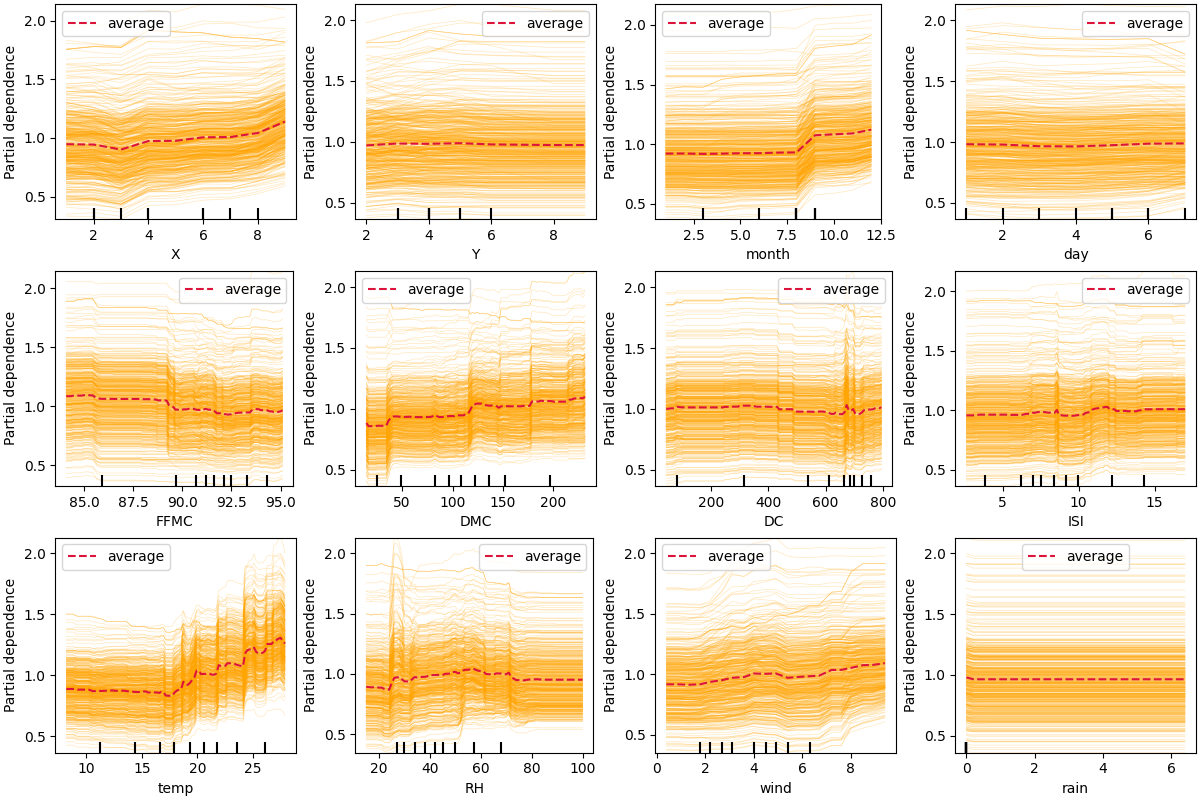
\includegraphics[width=\textwidth]{PDPs.png}
    \caption{Partial Dependence Plots for all variables using the XGBoost model}
    \label{fig:pdps}
\end{figure}

Figure \ref{fig:pdps} paints a much more complete picture of how the individual features are related to the outcome. While some features like \texttt{Y}, \texttt{day} or \texttt{rain} (which also had the lowest feature importances) show relatively constant lines, the other features show much more nuanced interaction. As expected, as \texttt{temp} increases, predictions increase, but the interaction is not as linear as one might expect. Similarly, \texttt{month}, \texttt{DMC} or \texttt{RH} show more intericate interactions. Moreover, the relative humidity \texttt{RH} first has prediction values increasing, before flattening out again, indicating that very low humidity actually decreases the expected area of forest fires, given the XGBoost model's fit.

Because a lot of values of the log area are 0, I further investigated whether classifier models could be of use, predicting whether a fire might take place or not (binary outcomes of 0 and 1). However, both logistic regression and the classifier version of XGBoost performed badly, resorting to constant predictions of 0. Investigating the probability predicted by the models, that too is constant at around 45\%. Looking at the distribution of the data (figure \ref{fig:hist_area}), a lot of values are very close to 0, so differentiating between exact 0 value or slightly higher proved too difficult. In general the regression models performed substantially better and should thus be preferred, as they can still predict very low values of area if it appears unlikely but is not constrained by a simple yes or no. Additionally, even a small difference between 0 and 0.1 makes a big difference in the response and potential area burned, so zero predictions of the classifiers are undesirable. When using the model to predict the likely area or size of a fire given input data, the regression models thus offer a much more complete and accurate picture of the outcome than the classification models could. 


\section{Location of forest fires}


Using the XGB model for predictions, it is now possible to investigate which areas are most at risk of fires (a larger predicted area), given input features. The simplest way is to set all variables at their mean and then plot the predicted area for each coordinate pair. Figure \ref{fig:pred_area_map} shows these predictions.

\begin{figure}[!htbp]
    \centering
    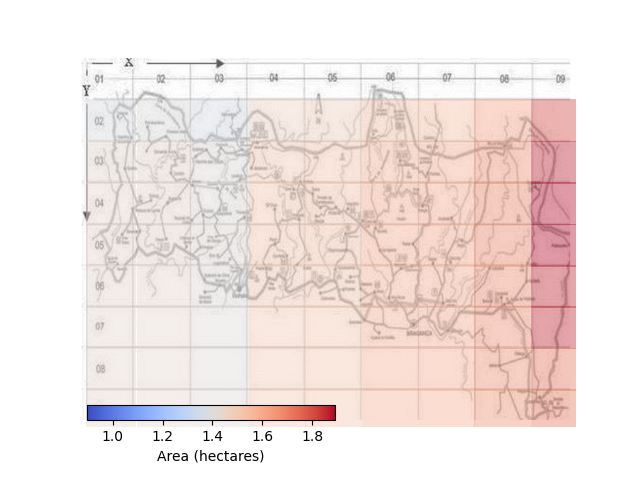
\includegraphics[width=\textwidth]{pred_area_map.png}
    \caption{Predicted outcome per coordinate pair, XGBoost}
    \label{fig:pred_area_map}
\end{figure}

Looking at the predicted outcome per coordinate rectangle, we can see that prediction values increase as \texttt{X} increases (towards the east). Values on the west side of the park have comparatively low values. Comparing this to the incidents on the map in figure \ref{fig:map_fires}, there are relatively few fires in the west and the majority seems to be concentrated around the center to east area. So if all features are at their respective mean values, the eastern side of the park is at much higher risk.

Another way is to compute the expected area per coordinate pair in a similar fashion as the ICE. For each (\texttt{X}, \texttt{Y}) pair, the model can predict the area for each observation in the dataset, just substituting in the respective coordinates. However, this full data pass lead to relatively constant predictions, as the outcomes were all around 1.52-1.53. This could be because other features are much more relevant so averaging over all the data will always lead to relatively similar predictions. 
%Figure \ref{fig:pred_area_map_full} shows these predictions.
%\begin{figure}[!htbp]
%     \centering
%     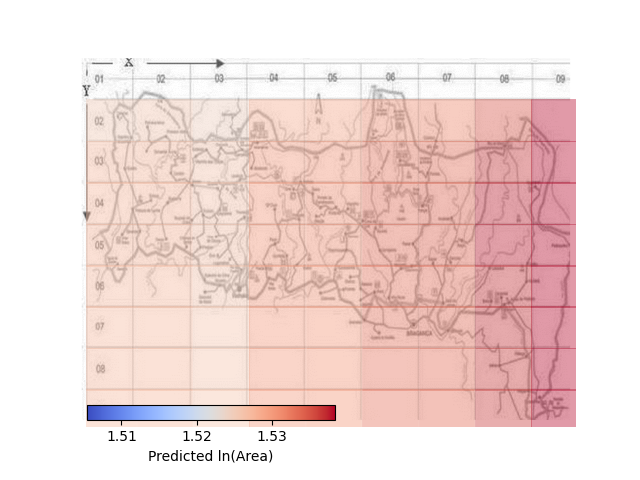
\includegraphics[width=\textwidth]{pred_area_map_full.png}
%     \caption{Predicted outcome per coordinate pair, XGBoost, full data pass}
%     \label{fig:pred_area_map_full}
% \end{figure}
% COULD SCRAP, JUST MENTION AND SAY AVG NOT VERY HIGH EFFECT AND ALL RELATIVELY CONSTANT PREDS

To investigate how the predicted area changes as more extreme feature values are observed, the map can be plotted for feature values that should produce very low or high output. To do this, I selected the feature values which had the lowest and highest partial dependence in figure \ref{fig:pdps}, meaning each feature at the value which individually leads to the lowest/highest model predictions. Figure \ref{fig:map_high_low} shows these maps.

\begin{figure}[!ht]
\centering 
\begin{subfigure}{0.48\textwidth} 
    \centering 
    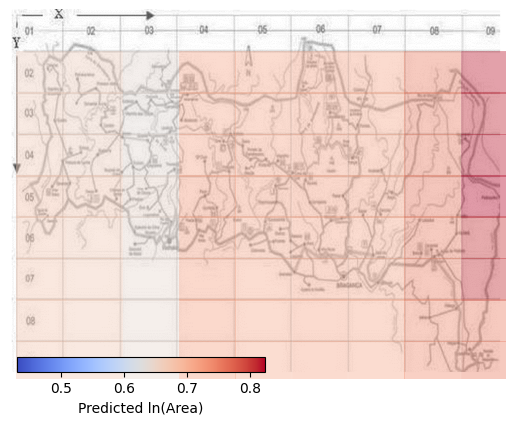
\includegraphics[width=1.05\linewidth]{map_lowest.png} 
    \caption{Lowest} 
    \label{fig:map_lowest} 
\end{subfigure} 
\begin{subfigure}{0.48\textwidth} 
    \centering
    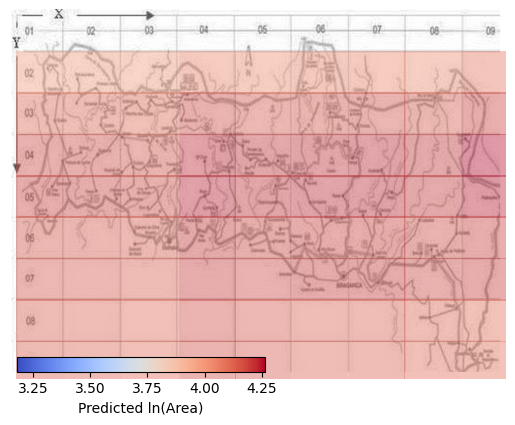
\includegraphics[width=1.05\linewidth]{map_highest.png} 
    \caption{Highest} 
    \label{fig:map_highest} 
\end{subfigure}
\caption{Predicted outcome per coordinate pair, setting feature values to minimizing and maximizing values}
\label{fig:map_high_low}
\end{figure}

As expected, the predicted outcome (transformed back to original scale in hectares) differs significantly. While in the plot with lowest values, the maximum values are around 0.8 hectares, for the other map that is around 4.2 hectares (over five times as much). Still, for both of these plots, the predicted values increase towards the center/right side of the map, although the map with maximizing inputs looks closer to the original map of forest fires. That the map with minimizing inputs has such a strong increase along the x-coordinates, could indicate that for generally adverse conditions for fires, rectangles towards the east end of the map are at higher risk of fires.

The publicly available code also contains a file called \texttt{forecast.py} in the folder \texttt{analyses}, which allows the user to specify input features and have either the whole map plotted, or the area for a specific rectangle returned. Also available are the function calls used to generate the plots with minimizing and maximizing feature inputs.

\section{Conclusion}
In conclusion, this article showed how to use machine learning models to predict forest fires and understand the main causes. As a first step, it is important to get an understanding of the dataset and the relation of the outcome variable with the features, potentially transforming the data in some way if necessary.

After understanding the models used, tuning the hyperparameters with Bayesian Optimization or grid search provides a way of finding the best model specifications. Apart from that, a KS test can be used to determine the most likely data distribution and use that for a generalized linear model.

After comparing the models in terms of predictive power in section 3.1, either regression coefficients, built-in feature importance tools or partial dependence plots can be used to understand how each variables influences the outcome. Here, the month, temperature and humidity of the environment (\texttt{DC)} were the most important variables. Additionally, the center and east end of the park seemed to be at higher risk of forest fires. Finally, this project investigates the most likely locations of forest fires and provides a tool to show the map for specified inputs. The code for all of this is available, so feel free to experiment with the setup, different models, or the interactive map!

\bibliography{References}

\end{document}
